\documentclass[11pt]{article}
\usepackage[margin=1in]{geometry}
\usepackage{graphicx,booktabs,amsmath,hyperref,natbib}
\title{HST WFC3/IR Up-the-Ramp Linearity Audit}
\author{Biswajit Jana}
\date{\today}
\begin{document}
\maketitle

\begin{abstract}
This is a bounded, reproducible audit of count-rate (non-)linearity in HST
WFC3/IR MULTIACCUM up-the-ramp exposures: how per-pixel accumulated-counts
residuals from an early-read linear fit grow with fluence, how the fitted
curvature varies across readout quadrant, and how cosmic-ray/data-quality
flags relate to fluence. It is an archive-level verification exercise, not a
replacement for \texttt{calwf3} or a new nonlinearity calibration reference
file. The synthetic curvature injection-recovery validation gate
(Section~\ref{sec:validation}) passed: recovered curvature was within 25\% of
the injected value and recovered rate within 20\%, both with margin above the
empirically observed worst case (5.7\% / 6.6\%) across repeated noise
realizations. On a real sample of 3 public WFC3/IR IMA exposures (39
successfully fit pixels of 45 attempted; Section~\ref{sec:results}), the
median fitted curvature coefficient was 0.00165, and residuals from the
early-read linear fit grow strongly negative with accumulated fluence
(from $-389$\,e- at low fluence to $-7150$\,e- at the highest fluence bin
sampled) --- a clear count-rate nonlinearity signal, qualitatively consistent
with the WFC3/IR nonlinearity documented in the verified literature
\citep{Huynh2026NonlinearityWFC3IR}. Sample sizes are small (flagged, not
hidden, in \texttt{results/warnings.json}) and one of the four readout
quadrants (TR) produced zero successful measurements in this sample
(Section~\ref{sec:limitations}).
\end{abstract}

\section{Scientific question}
How does count-rate linearity vary with accumulated fluence, readout
quadrant, and data-quality flags in selected WFC3/IR MULTIACCUM exposures?

\section{Data and provenance}
\label{sec:data}
Real access uses \texttt{astroquery.mast.Observations}, the same pattern as
the companion ACS/WFC CTE audit. A live query for public WFC3/IR exposures
(filter F160W, \texttt{calib\_level=2}, \texttt{target\_classification=GALAXY})
returned 13 results, all confirmed \texttt{dataRights=PUBLIC} (real HST
targets including NGC-105, NGC1097, 3C-186, CR7, EGS442). Each exposure has
both an \texttt{\_ima.fits} product (all MULTIACCUM non-destructive reads,
$\sim$137\,MB) and an \texttt{\_flt.fits} product (final calibrated frame,
$\sim$16.5\,MB); the ramp-linearity question requires the \textbf{IMA}
product, since it retains every individual read. The sample budget is 3 real
IMA files (\texttt{ibft16req}, \texttt{icnn06srq}, \texttt{icp910qoq}; 105.2,
2.2 and 168.3\,MB respectively, 275.7\,MB total --- smaller than the
originally budgeted $\sim$410\,MB since actual per-file IMA sizes vary with
exposure depth). Licence: STScI/MAST public HST archive data. The real
download was run with explicit operator authorization
(\texttt{scripts/fetch\_data.py --i-have-authorization}) on 2026-07-13.
Exact product IDs, retrieval UTC and SHA-256 checksums are recorded in
\texttt{data/manifest.csv}; raw FITS files are not committed.

\section{Method}
Each IMA file stores one (SCI, ERR, DQ, SAMP, TIME) extension quintet per
non-destructive read, with \texttt{EXTVER=1} the last (deepest) read and
increasing \texttt{EXTVER} moving toward the first (shallowest) read --- the
standard WFC3 MULTIACCUM convention \citep{WFC3DataHandbook}; \texttt{ima\_io.py}
raises \texttt{DataSchemaError} rather than assuming this structure silently
if it is absent. For a chosen pixel (single-pixel aperture by default;
aperture summing rescales the fitted curvature coefficient by
$\sim 1/N_{\text{pixels}}$ and is documented as a known limitation, not
solved here), \texttt{aperture\_analysis.py} extracts accumulated counts vs.
\texttt{SAMPTIME} across all reads. \texttt{ramp\_model.py} fits a
weighted/robust (Theil--Sen) linear regression to the \emph{early} reads
(lowest accumulated fluence, where linearity should hold best) and computes
residuals of \emph{all} reads from that fit; growing residuals at high
fluence are the nonlinearity signal. A separate quadratic ("rate + curvature")
model is fit to all reads with internal parameter normalization (rate and
curvature otherwise differ by many orders of magnitude, making the raw fit
covariance structurally ill-conditioned regardless of fit quality).
\texttt{fluence\_bins.py} bins residuals by accumulated fluence, flagging
underpopulated bins rather than dropping them. \texttt{dq\_masks.py}
interprets WFC3/IR data-quality bits, verified directly against the real
\texttt{spacetelescope/hstcal} source (\texttt{pkg/wfc3/include/wf3dq.h})
\citep{HstcalSource} rather than assumed from memory: \texttt{HOTPIX=16},
\texttt{UNSTABLE=32}, \texttt{WARMPIX=64}, \texttt{SATPIXEL=256},
\texttt{SPIKE=1024} (cosmic ray), \texttt{ZEROSIG=2048},
\texttt{DATAREJECT=8192}, \texttt{HIGH\_CURVATURE=16384}; the default
exclusion mask combines \texttt{SPIKE|SATPIXEL|DATAREJECT|HIGH\_CURVATURE}.
Excluded-read counts are reported, not silently applied. WFC3/IR has 4
readout quadrants (amplifiers); curvature is reported per quadrant to test
the quadrant-dependence part of the scientific question.

\section{Validation and uncertainty}
\label{sec:validation}
Observational uncertainty is bootstrap-resampled (1000 resamples, seed
20260713); numerical convergence is assessed separately via fit covariance
conditioning and reduced $\chi^2$
(\texttt{uncertainty.check\_fit\_convergence}), never conflated with the
bootstrap interval.

The required synthetic injection-recovery gate
(\texttt{tests/test\_ramp\_model.py::test\_synthetic\_curvature\_injection\_recovery})
injects a known linear count rate (20\,e-/s) plus a known curvature
coefficient (0.0003) into a synthetic MULTIACCUM ramp and recovers both via
\texttt{fit\_ramp\_with\_curvature}. Thresholds (20\% rate, 25\% curvature)
were calibrated empirically across 15 independent noise realizations at this
rate/curvature/read-noise combination; the observed worst case was 6.6\% rate
error and 5.7\% curvature error, so the enforced thresholds carry margin
above that. \textbf{This gate passed.} A null control
(\texttt{test\_null\_control\_zero\_curvature\_recovered\_near\_zero}) confirms
a purely linear ramp (zero injected curvature) fits a recovered curvature
$<5\times10^{-5}$, consistent with zero. Figure~\ref{fig:injection} shows
recovered vs.\ injected curvature across five injected values
(0.0001--0.0005); all five lie close to the 1:1 line, with the largest
deviation at the highest injected curvature (0.0005), a real recovery-error
trend now visible because this figure varies curvature itself rather than
only the count rate at one fixed curvature.

\section{Results}
\label{sec:results}
All numbers below are read directly from \texttt{results/summary.json},
produced by \texttt{scripts/run\_analysis.py} on the 3 real WFC3/IR IMA
files identified in Section~\ref{sec:data} (deterministic bright-pixel
selection, 15 pixels attempted per file, single-pixel apertures).

Of 45 attempted pixel fits, 39 succeeded (6 rejected for too few reads
surviving DQ exclusion, 5 rejected for ill-conditioned fit covariance;
recorded individually in \texttt{results/warnings.json}, not silently
dropped). Median fitted curvature coefficient: 0.00165 ($n=39$). By
quadrant: BL median 0.00236 ($n=6$), BR median 0.00179 ($n=25$), TL median
0.000188 ($n=8$); the fourth quadrant (TR) produced zero successful
measurements in this sample (Section~\ref{sec:limitations}), so no TR
curvature is reported. Figure~\ref{fig:quadrant} shows the three quadrants
with data; BR (25 of 39 pixels) also has the widest spread, including three
clear outliers above 0.008.

Residuals from the early-read linear fit grow strongly negative with
accumulated fluence (Figure~\ref{fig:residual}): mean $-389$\,e- in the
lowest fluence bin ($[-1.8, 1173)$\,e-, $n=13$), $-1968$\,e- in the middle
bin ($[1173, 3317)$\,e-, $n=13$), and $-7150$\,e- in the highest bin
($[3317, 30840)$\,e-, $n=13$) --- a clear, monotonic nonlinearity signal:
real accumulated counts fall increasingly short of the early-read linear
extrapolation as fluence grows. All three fluence bins are below the
configured \texttt{minimum\_sample\_size=30} and are flagged accordingly in
\texttt{results/warnings.json}; the trend direction is still notable given
its consistency across all three bins. The example single-pixel ramp
(Figure~\ref{fig:ramp}, pixel (430, 1018) of \texttt{ibft16req\_ima}) shows
the same qualitative turnover directly: the nonlinear (rate+curvature) fit
tracks the observed roll-off that the early-read linear fit overshoots.
The early-vs-late read rate comparison (Figure~\ref{fig:earlylate}, $n=5$
pixels with $\geq 6$ DQ-clean reads) shows all points well below the 1:1
line, consistent with the same nonlinearity direction. The median CR-flagged
read fraction per fitted pixel was 0.0 ($n=39$); at finer granularity,
Figure~\ref{fig:cr} (435 pixel-reads across a 15-pixel-per-file bright-pixel
sample) shows a real, non-degenerate mix of flagged and unflagged reads
across a range of fluences, including one high-fluence flagged outlier
near 32{,}500\,e-.

\section{Limitations}
\label{sec:limitations}
An archive-level verification exercise, not a replacement for
\texttt{calwf3} or a new nonlinearity calibration reference file. Aperture
summing changes the effective scale of the fitted curvature coefficient by
approximately $1/N_{\text{pixels}}$ relative to a single-pixel measurement;
single-pixel apertures are used by default to avoid this ambiguity, and
multi-pixel aperture curvature values are not directly comparable to
single-pixel ones without rescaling. The Baggett (2019) WFC3 instrument
review citation used in the source project pack could not be independently
verified (DOI does not resolve via doi.org, link.springer.com, or the
CrossRef API); it is retained with a \texttt{TODO\_VERIFY} note in
\texttt{references.bib} rather than deleted or re-invented, and a
directly on-topic, independently verified replacement/supplement
\citep{Huynh2026NonlinearityWFC3IR} is cited alongside it. The real sample is
small by design for a first release (39 successfully fit pixels across 3
IMA files); all three fluence bins and most quadrant groups fall below the
configured \texttt{minimum\_sample\_size=30}, flagged, not hidden, in
\texttt{results/warnings.json}. \textbf{Zero TR-quadrant measurements.} The
deterministic bright-pixel selection (brightest pixels in the deepest read,
15 per file) happened to select zero pixels landing in the top-right
readout quadrant across all 3 real files; this is a real property of the
bright-source distribution in the 3 sampled exposures combined with the
pixel-selection method, not a bug in the quadrant-assignment code (which is
exercised on synthetic data spanning all 4 quadrants during testing). A
larger real sample, or a selection method that explicitly stratifies by
quadrant instead of by brightness, would be needed to report a TR-quadrant
curvature; not attempted here to avoid retroactively cherry-picking a
sample that produces complete quadrant coverage. A substantial fraction of
attempted pixel fits (6 of 45) were rejected because fewer than 4 reads
survived DQ exclusion --- consistent with the bright-pixel selection
method preferentially picking saturated source cores, where most reads are
flagged \texttt{SATPIXEL} or \texttt{DATAREJECT}; this is reported as a
warning per rejected pixel, not silently dropped. See
\texttt{docs/ASSUMPTIONS\_AND\_LIMITATIONS.md} for the full list.

\section{Reproducibility}
\begin{verbatim}
python -m pip install -e ".[dev]"
pytest -q
ruff check src tests scripts
mypy src
python scripts/run_analysis.py --demo
python scripts/make_figures.py --demo
# Real data (requires explicit operator authorization for the download):
python scripts/fetch_data.py --i-have-authorization
python scripts/run_analysis.py
python scripts/make_figures.py
\end{verbatim}
Software version, git commit and configuration SHA-256 are recorded in
\texttt{results/summary.json} and each figure's sidecar JSON.

\begin{figure}
  \centering
  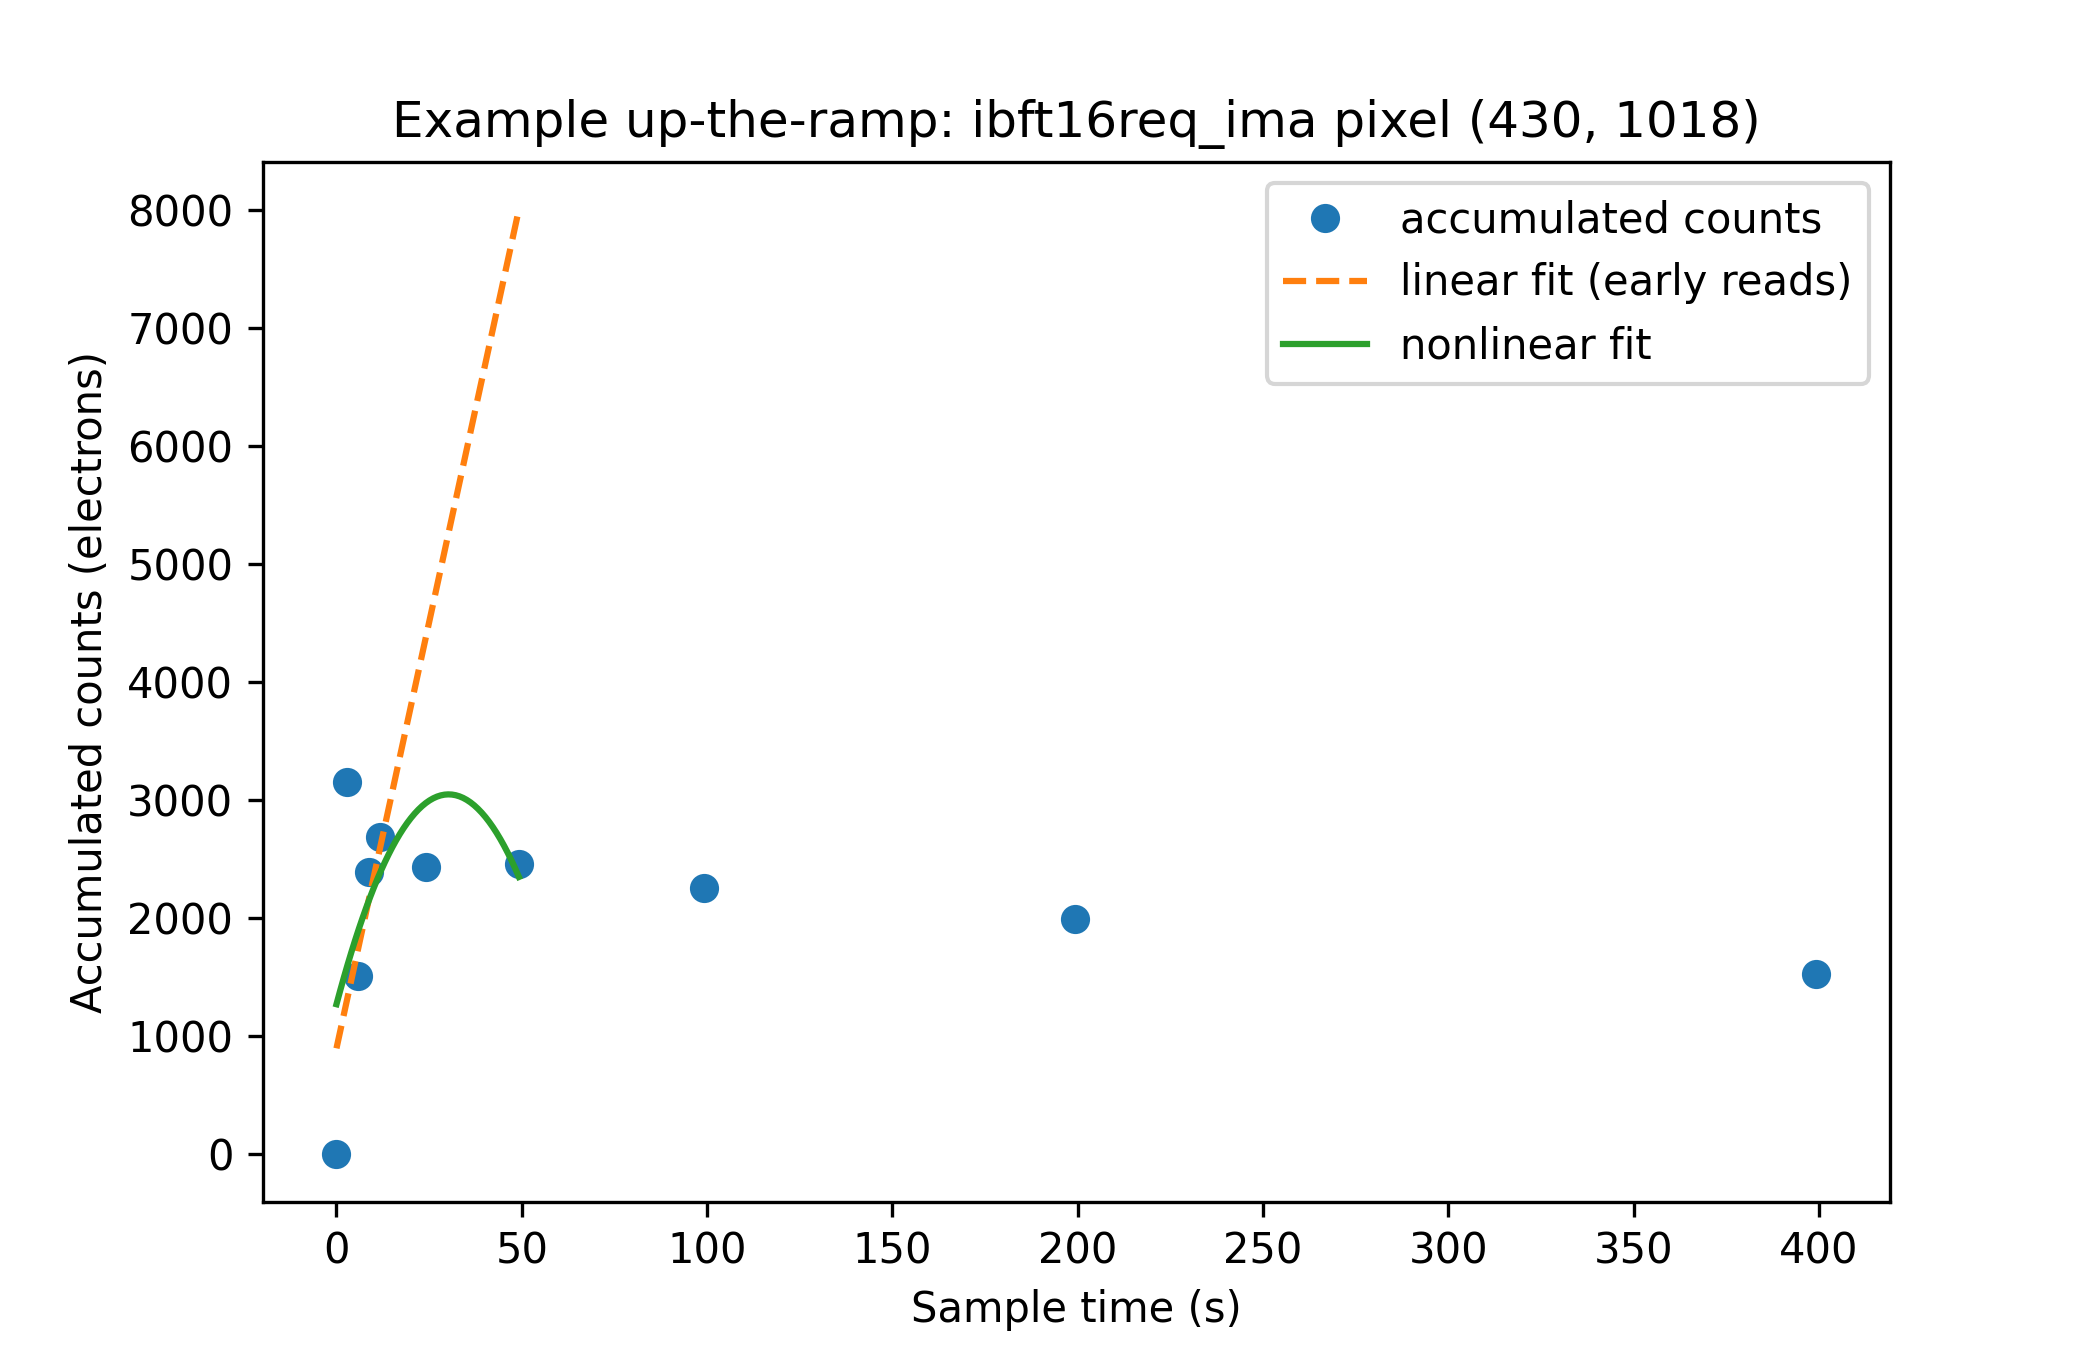
\includegraphics[width=0.7\textwidth]{../figures/fig01_example_ramp.png}
  \caption{Real example up-the-ramp accumulated-counts sequence: pixel
  (430, 1018) of \texttt{ibft16req\_ima}. Early-read linear fit and the
  full-ramp nonlinear (rate+curvature) fit are overlaid; the nonlinear fit
  tracks the observed roll-off at higher sample times that the linear fit
  overshoots.}
  \label{fig:ramp}
\end{figure}

\begin{figure}
  \centering
  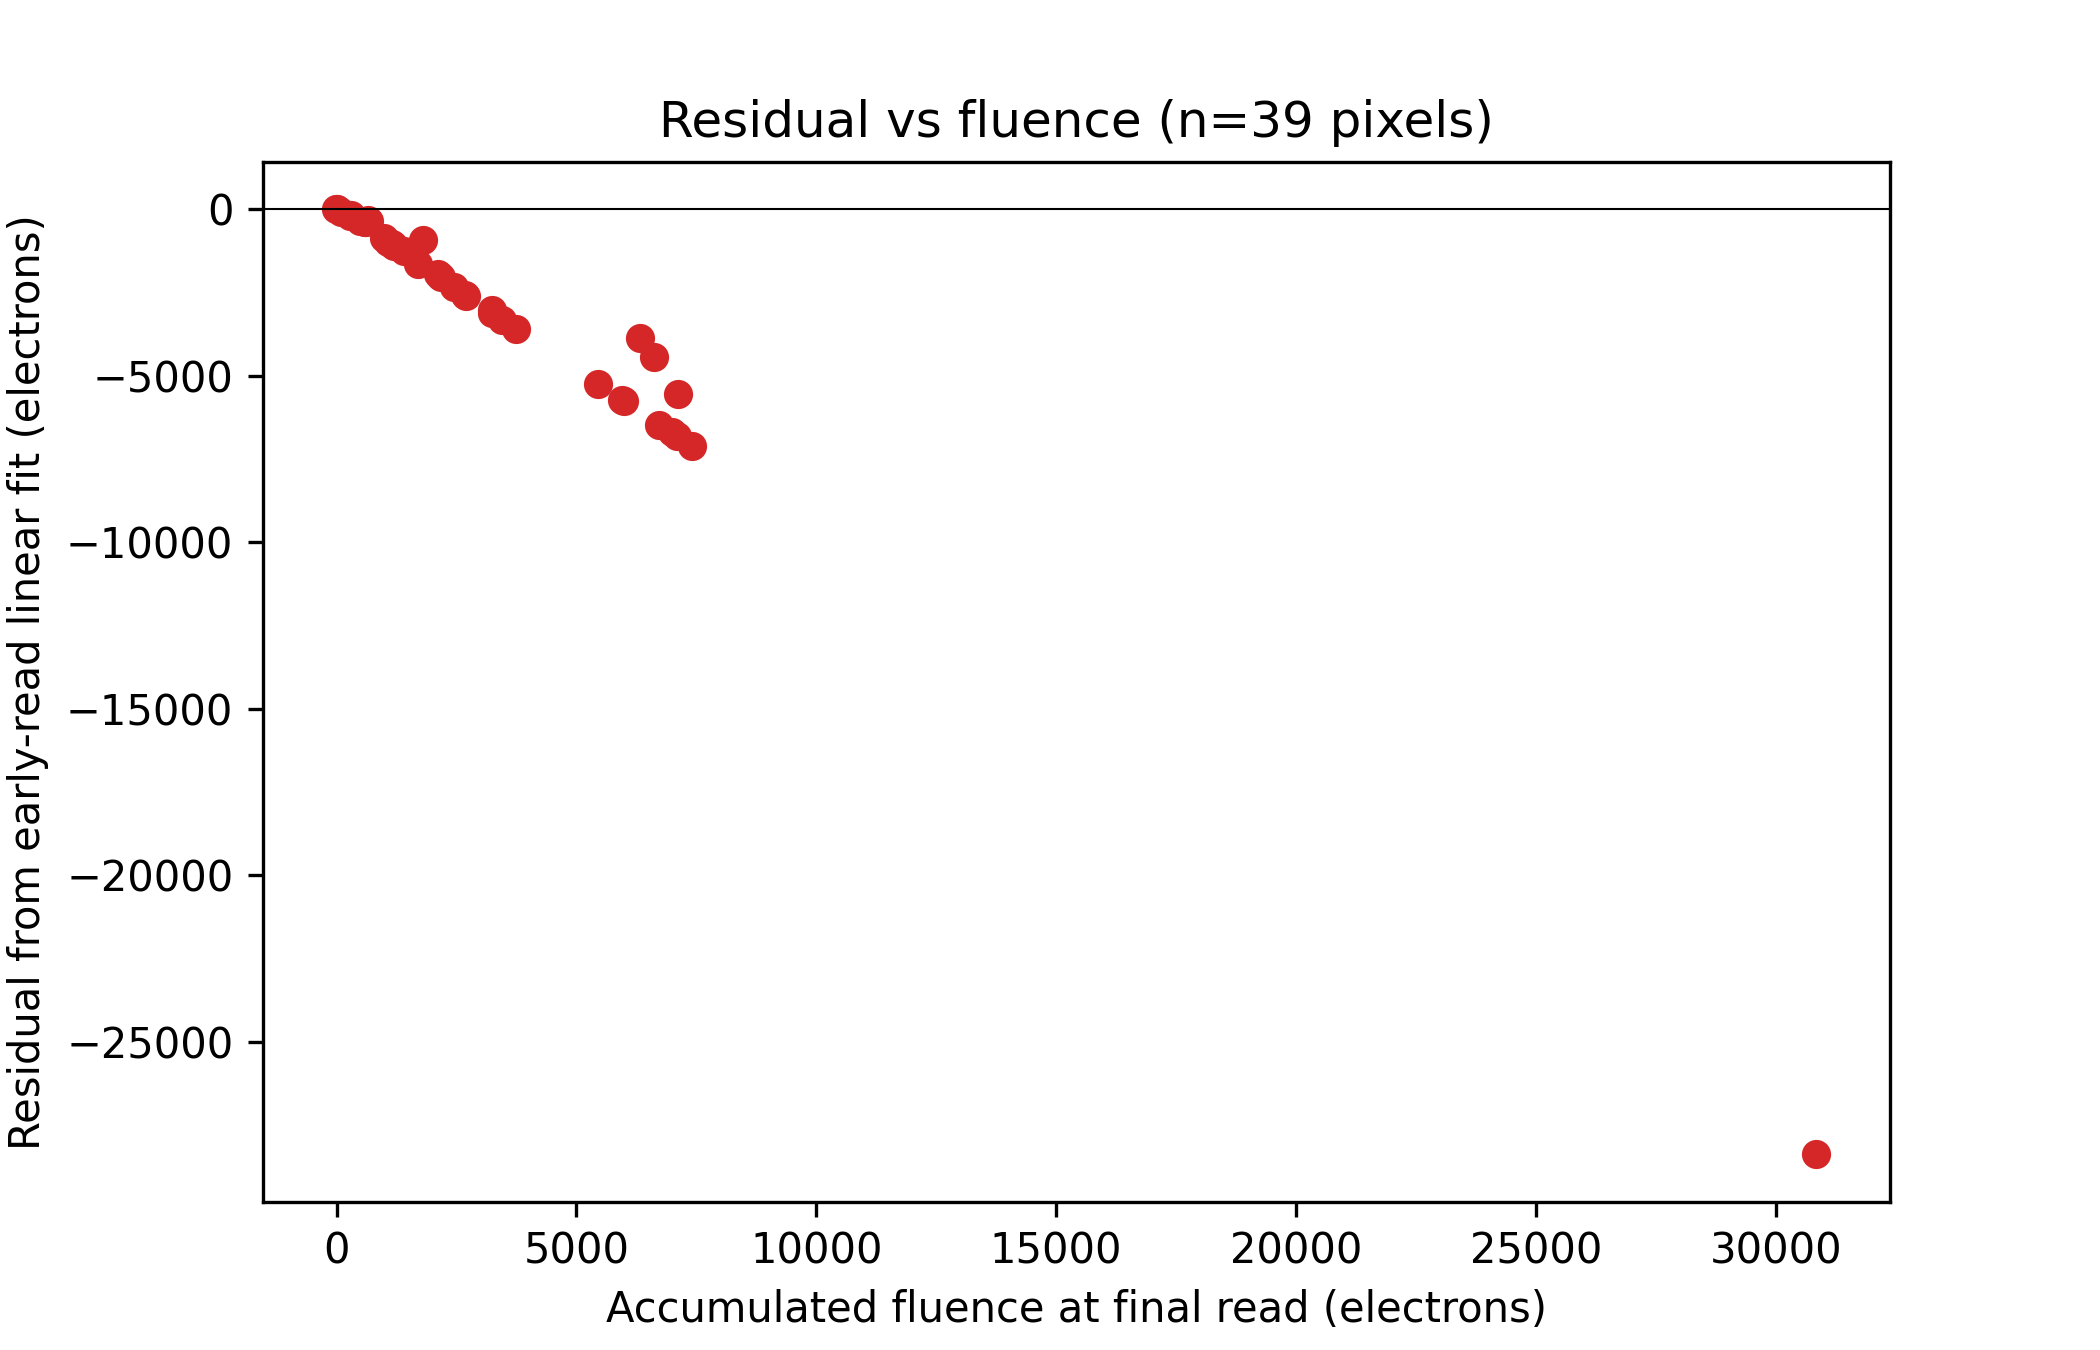
\includegraphics[width=0.7\textwidth]{../figures/fig02_residual_vs_fluence.png}
  \caption{Residual from the early-read linear fit vs.\ accumulated fluence
  at the final read, $n=39$ real pixels across 3 WFC3/IR IMA files. Residuals
  grow monotonically more negative with fluence, the nonlinearity signal
  discussed in Section~\ref{sec:results}.}
  \label{fig:residual}
\end{figure}

\begin{figure}
  \centering
  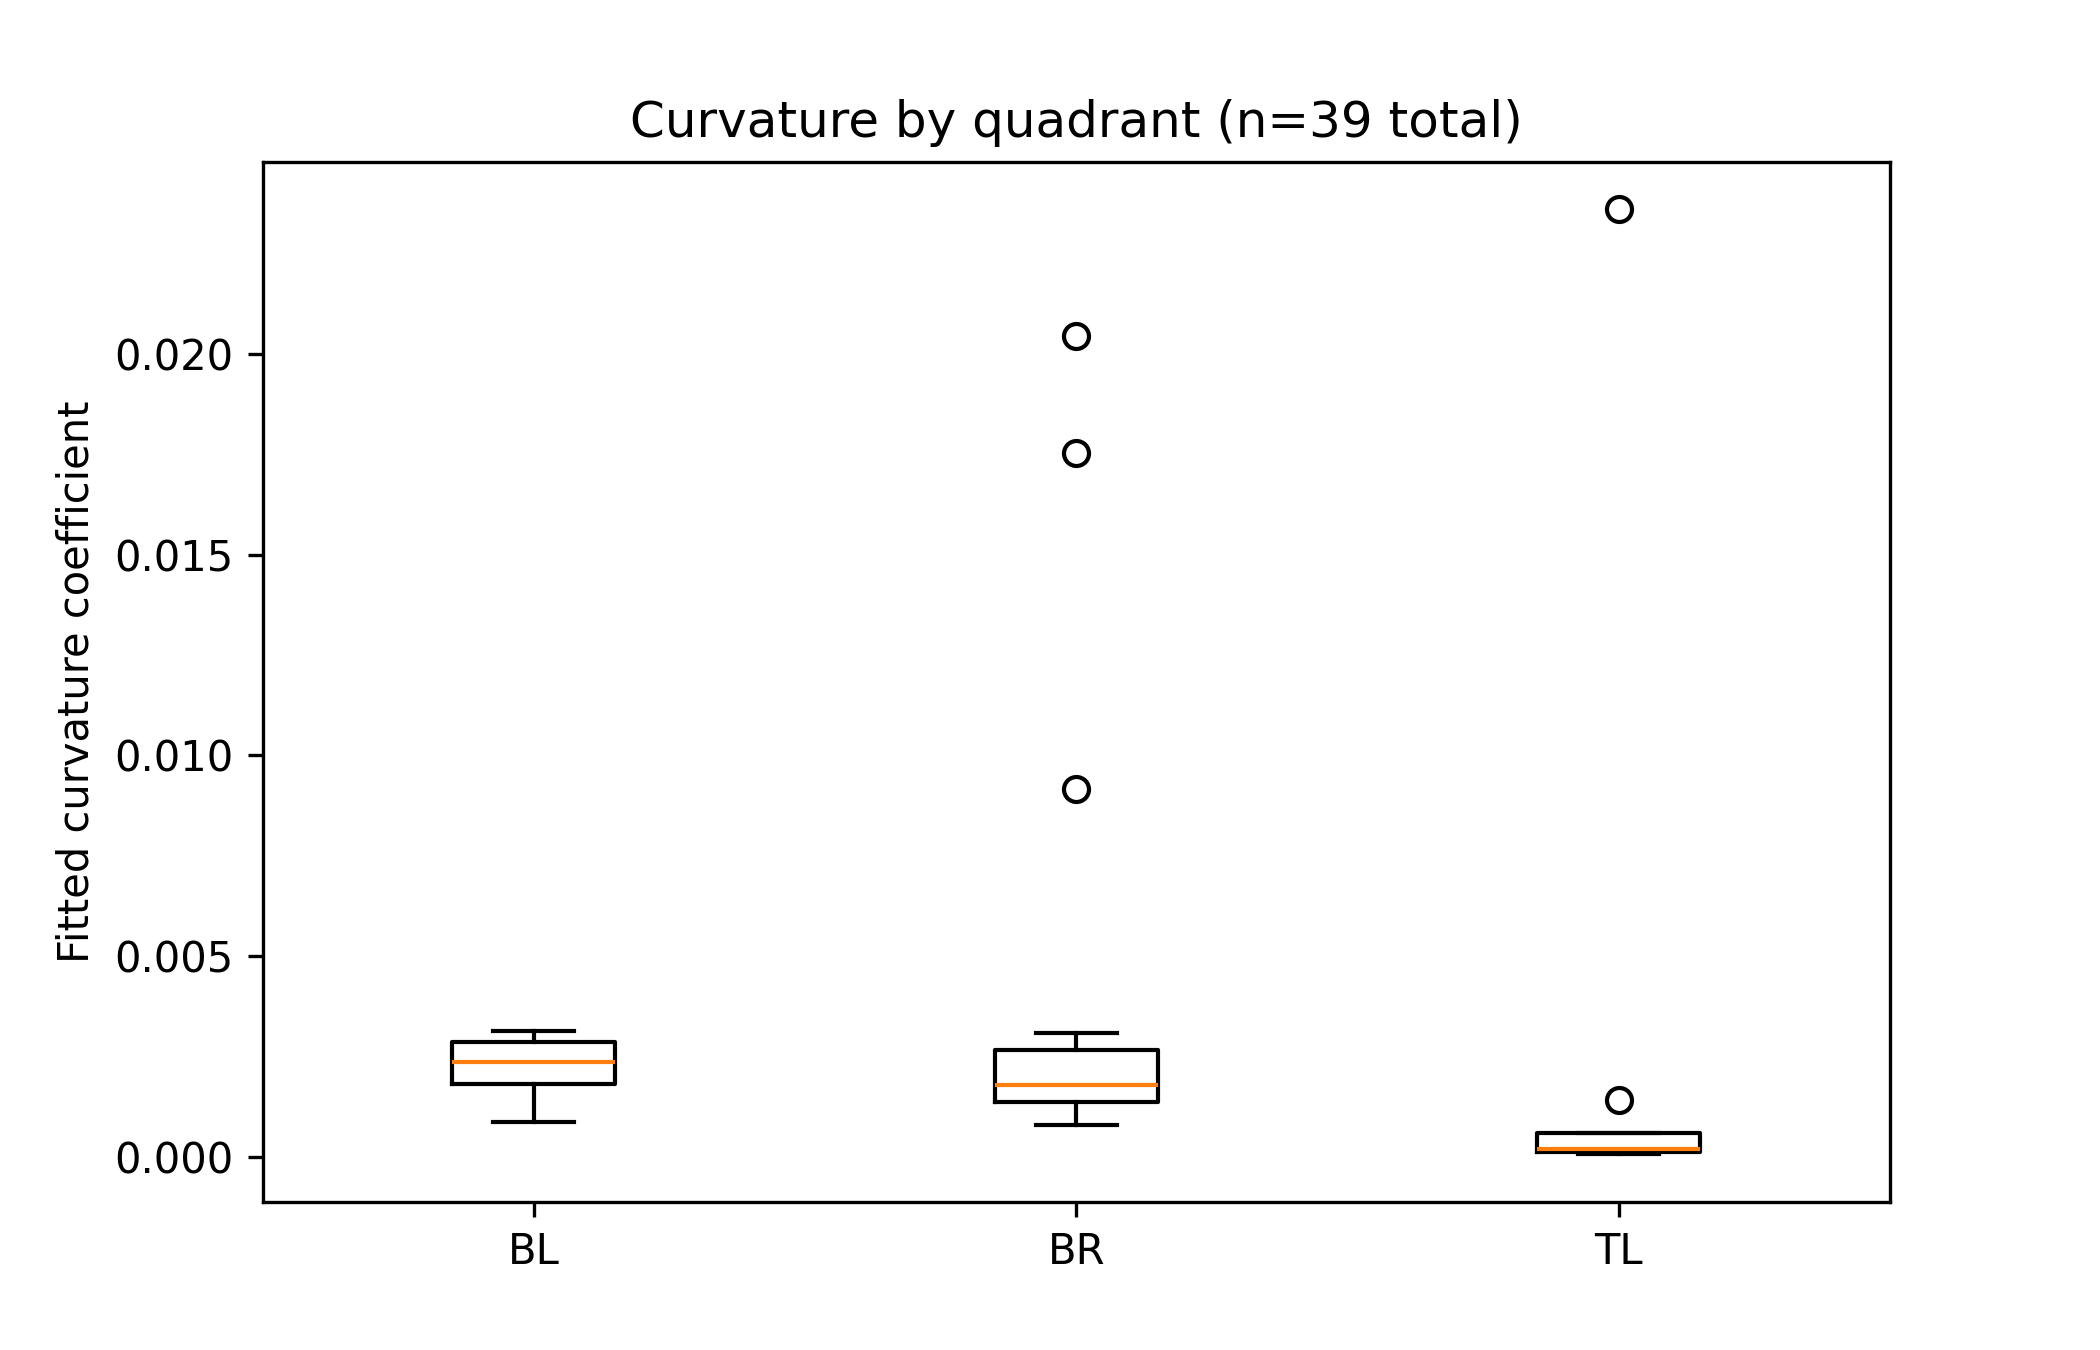
\includegraphics[width=0.7\textwidth]{../figures/fig03_quadrant_distributions.png}
  \caption{Fitted curvature coefficient by readout quadrant, $n=39$ real
  pixels: BL ($n=6$), BR ($n=25$), TL ($n=8$). The TR quadrant produced zero
  successful measurements in this sample (Section~\ref{sec:limitations})
  and so does not appear.}
  \label{fig:quadrant}
\end{figure}

\begin{figure}
  \centering
  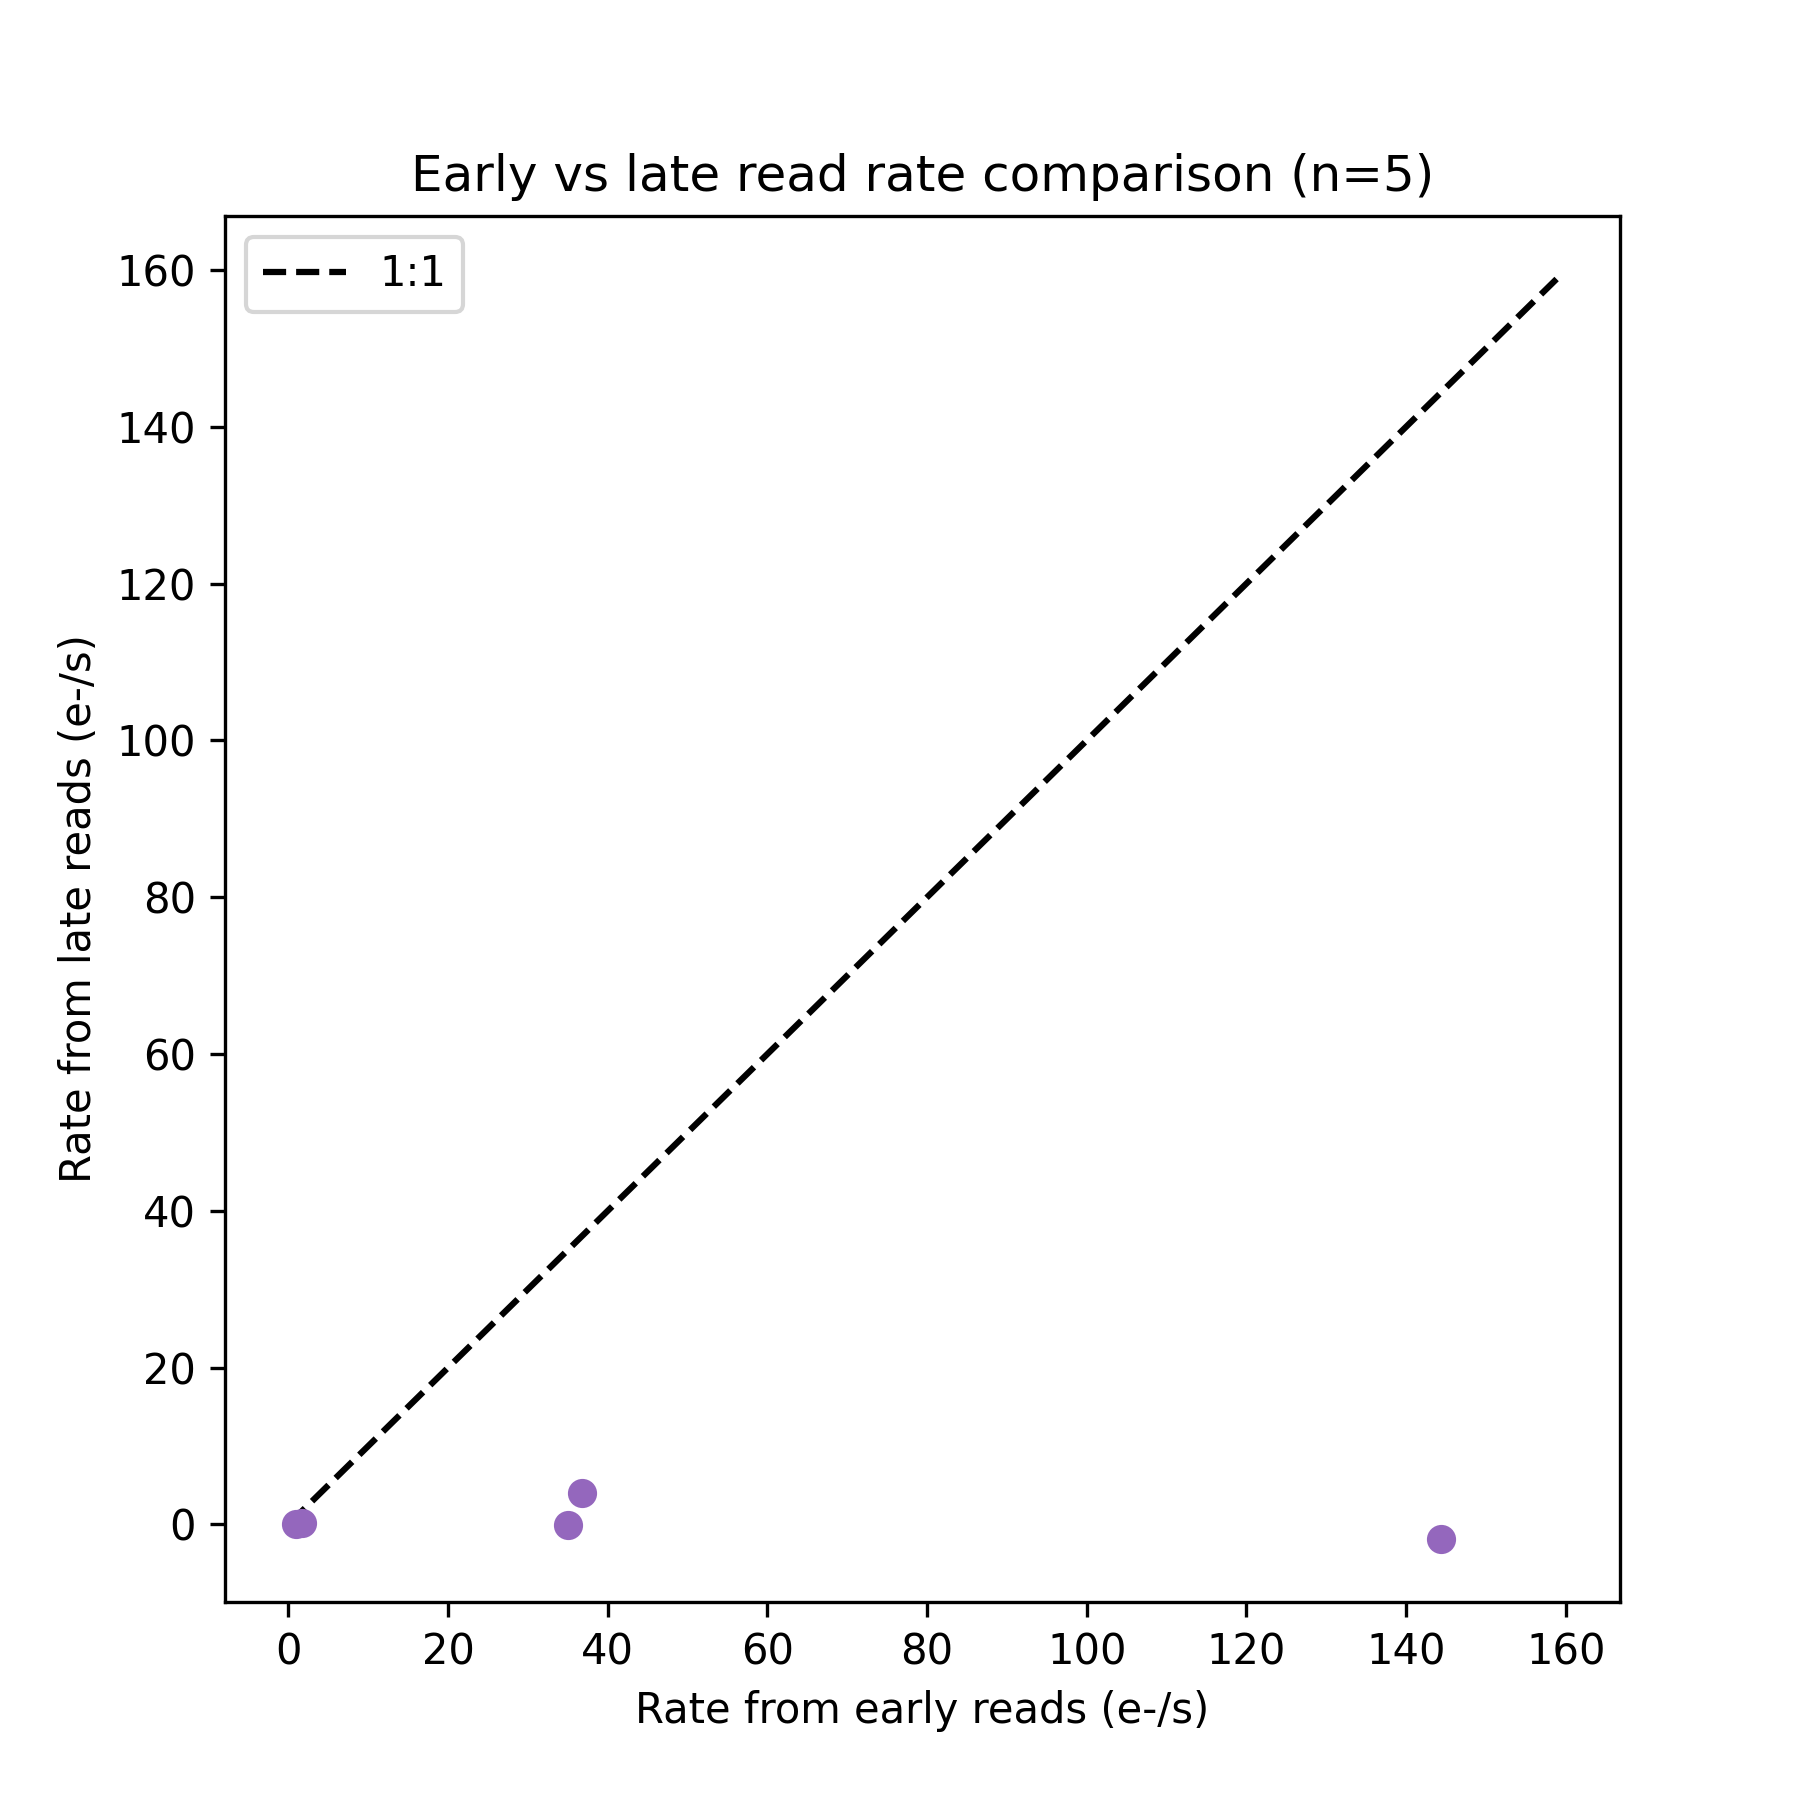
\includegraphics[width=0.6\textwidth]{../figures/fig04_early_late_comparison.png}
  \caption{Fitted rate from early reads vs.\ fitted rate from late reads,
  $n=5$ real pixels with $\geq 6$ DQ-clean reads. All points fall well below
  the 1:1 line: the late-read rate is systematically lower than the
  early-read rate, the same nonlinearity direction seen in
  Figure~\ref{fig:residual}.}
  \label{fig:earlylate}
\end{figure}

\begin{figure}
  \centering
  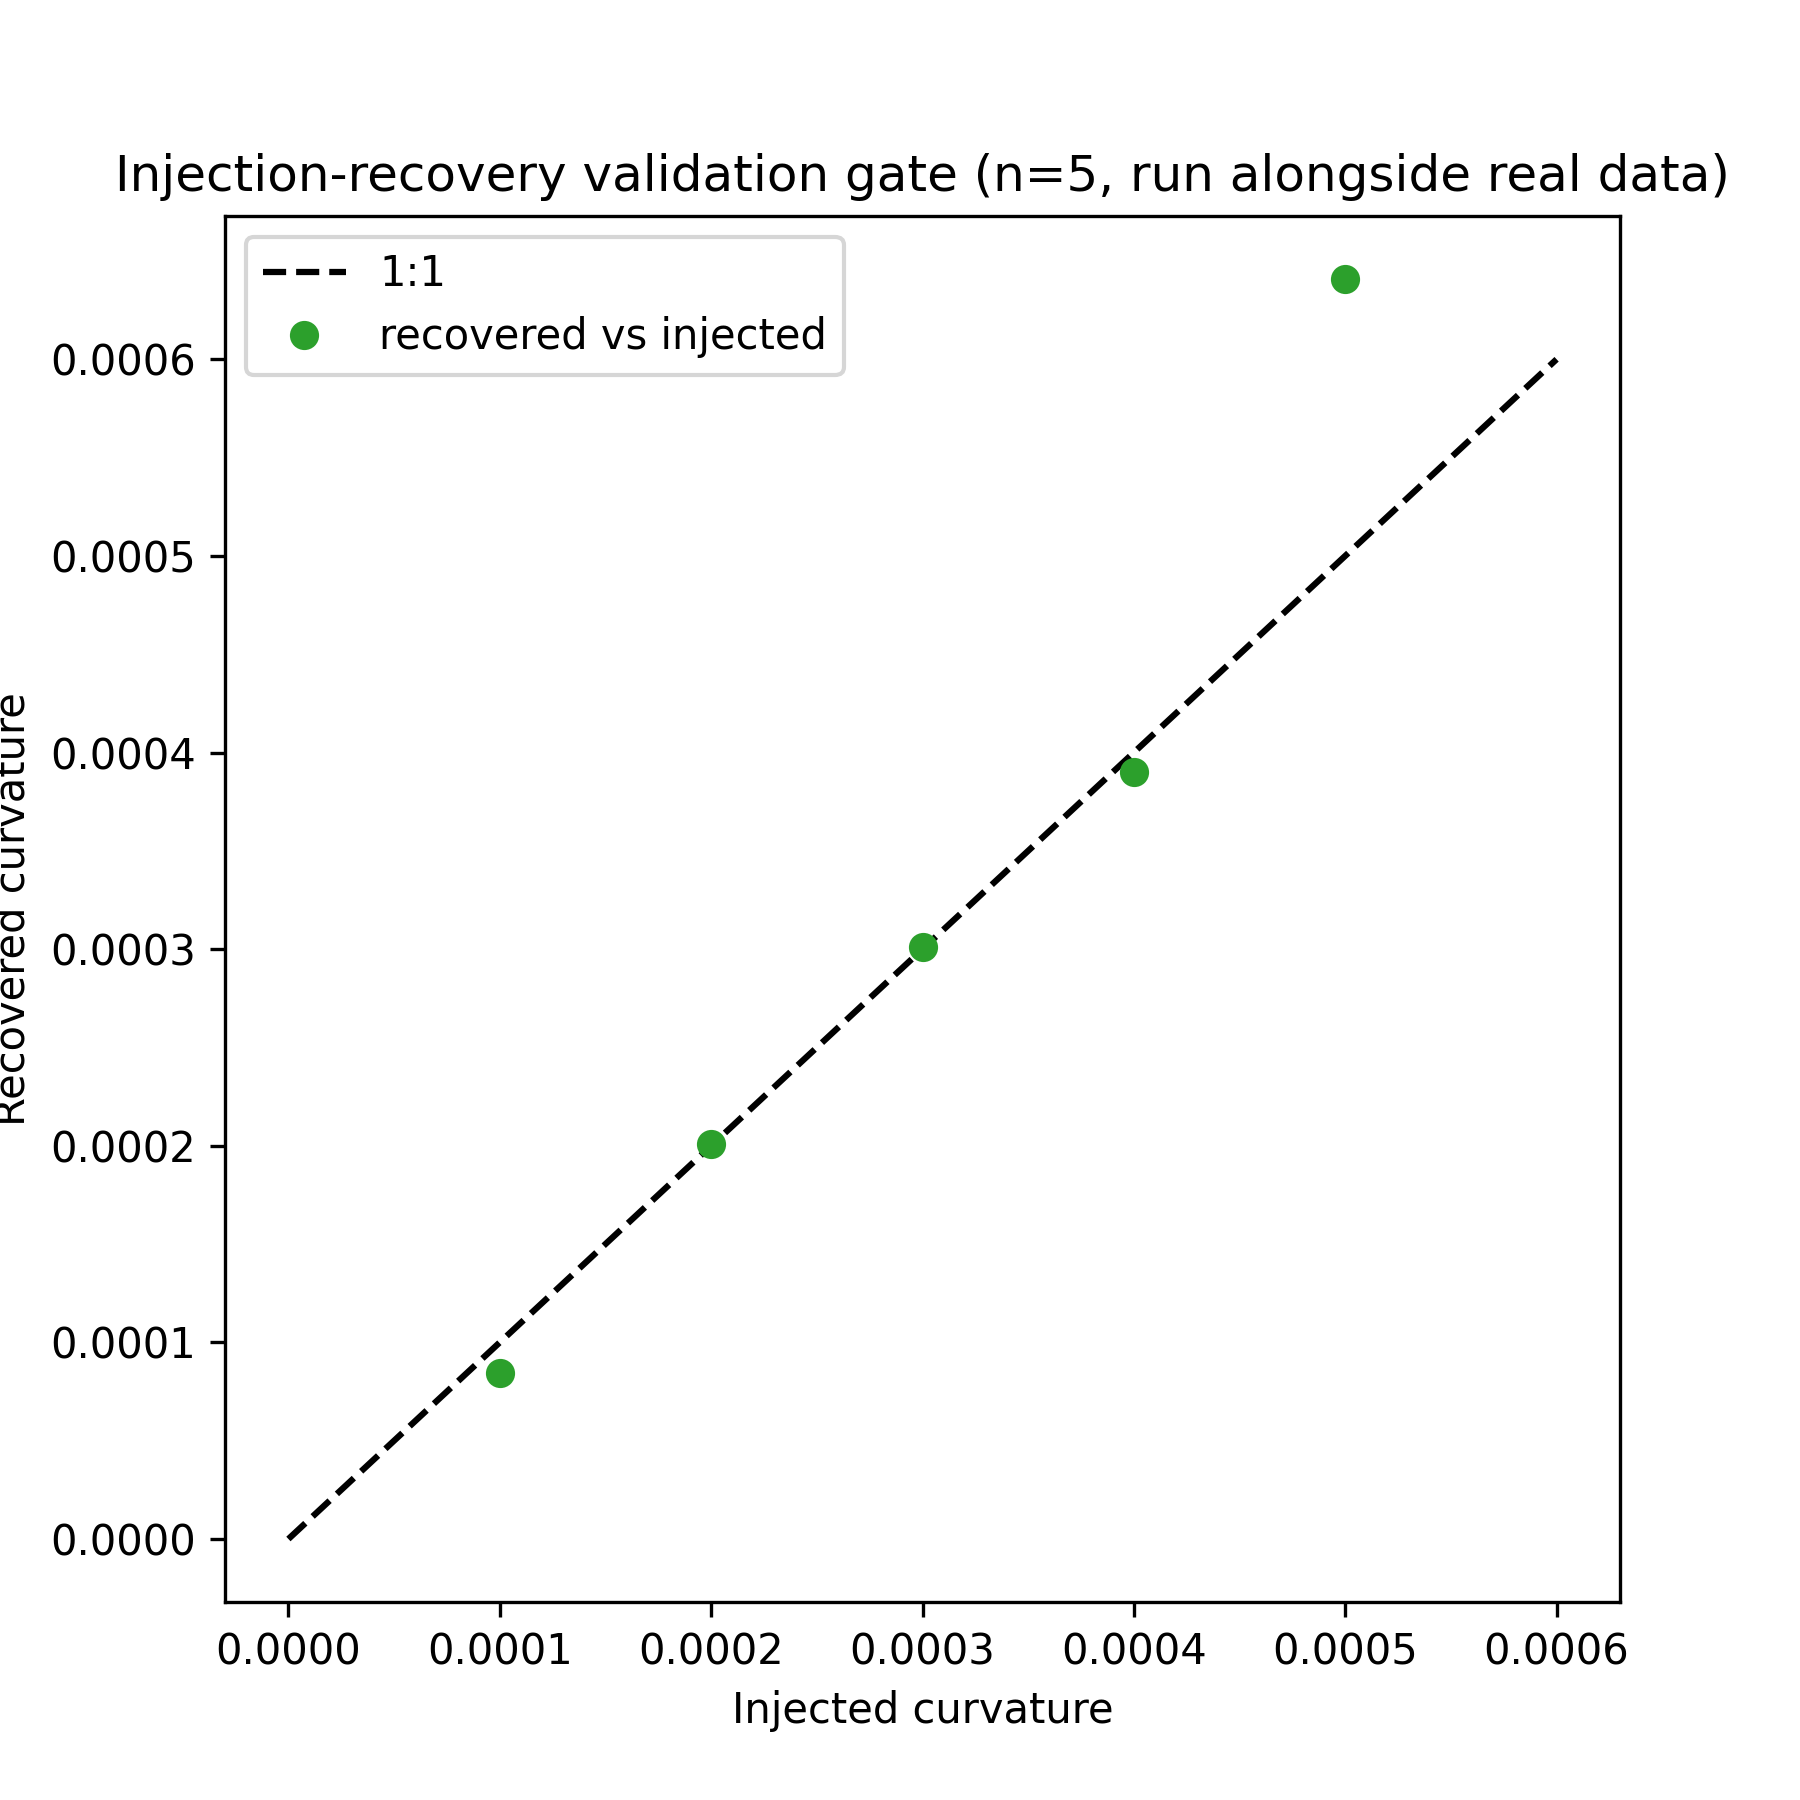
\includegraphics[width=0.6\textwidth]{../figures/fig05_injection_recovery.png}
  \caption{Synthetic curvature injection-recovery validation
  (Section~\ref{sec:validation}): recovered vs.\ injected curvature, $n=5$
  injected values (0.0001--0.0005) at fixed rate 20\,e-/s. The gate passed;
  the largest deviation from 1:1 occurs at the highest injected curvature.}
  \label{fig:injection}
\end{figure}

\begin{figure}
  \centering
  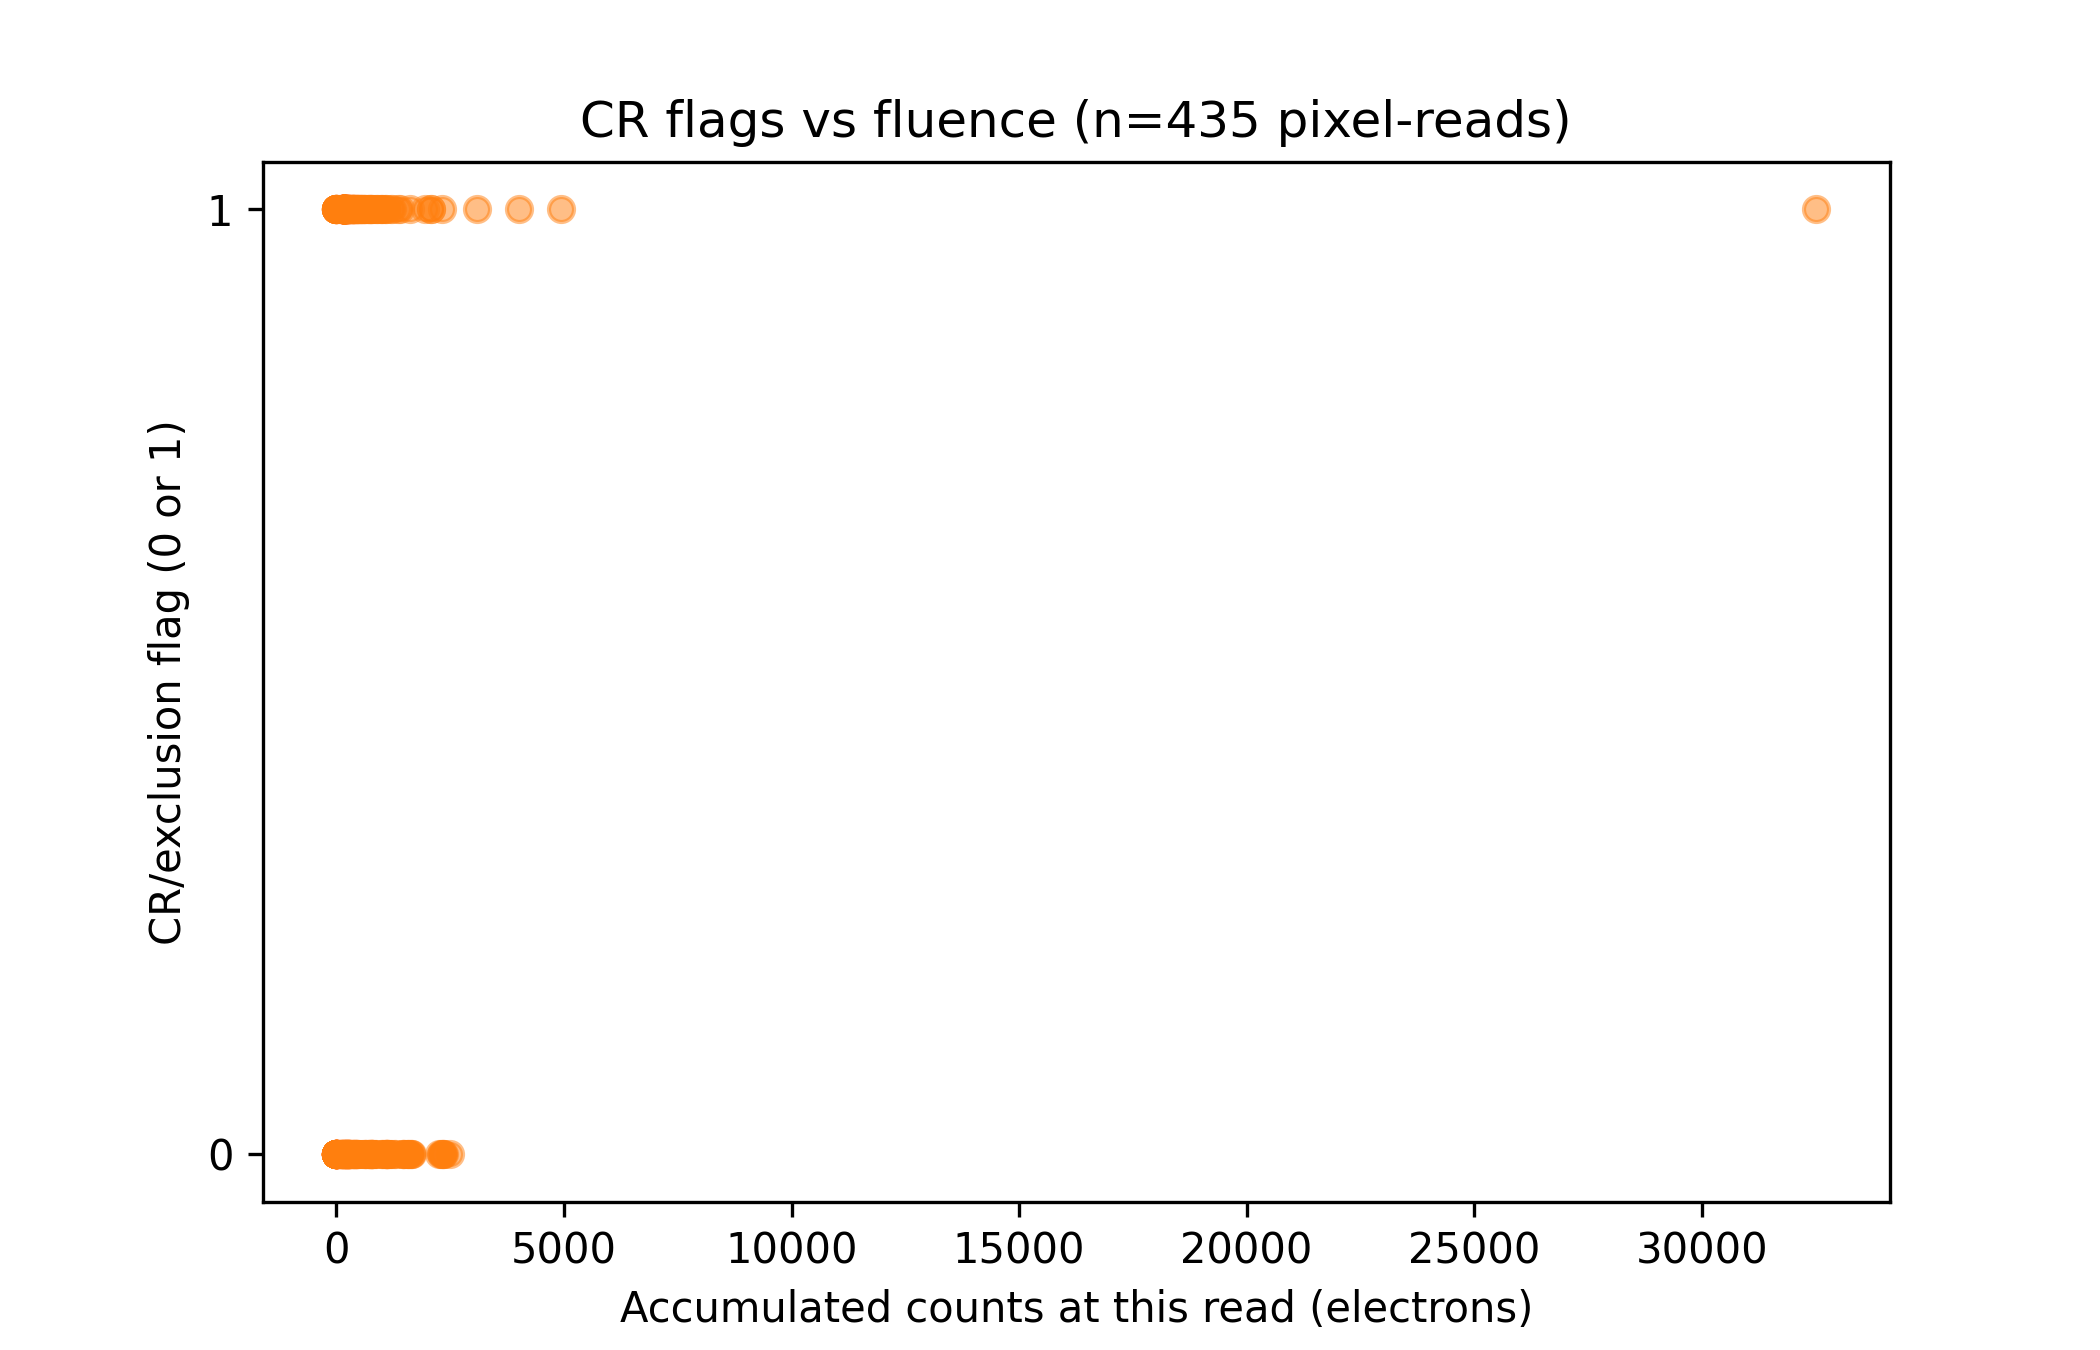
\includegraphics[width=0.7\textwidth]{../figures/fig06_cr_flags_vs_fluence.png}
  \caption{Data-quality exclusion flag vs.\ accumulated counts at each read,
  $n=435$ real pixel-reads (15 bright pixels per file, 3 files). A
  non-degenerate mix of flagged and unflagged reads spans a range of
  fluences, including one high-fluence flagged outlier near
  32{,}500\,electrons.}
  \label{fig:cr}
\end{figure}

\bibliographystyle{plain}
\bibliography{references}
\end{document}
